\documentclass{beamer}

\usepackage{hyperref}
\usepackage{bm}
\hypersetup{
  pdfinfo={
    CreationDate={D:20180702102722},
    ModDate={D:20180702102722},
  },
}

\definecolor{seaborn-blue}{HTML}{4B72B0}
\definecolor{seaborn-green}{HTML}{55A868}

\AtBeginSection[]
{
  \begin{frame}
    \frametitle{Table of Contents}
    \tableofcontents[currentsection]
  \end{frame}
}

\usetheme{metropolis}
% Some configurations of metropolis theme
\metroset{block=fill}
\metroset{numbering=none}
% Set some custom colors for the beamer theme
\definecolor{DarkBlue}{HTML}{163a7a}
\definecolor{jr@medblue}{RGB}{103,169,207}
\definecolor{jr@green}{RGB}{77,175,74}
\definecolor{jr@darkred}{RGB}{153,0,0}
\setbeamercolor{frametitle}{bg=DarkBlue}
\setbeamercolor{progress bar}{fg=black}
\setbeamercolor{progress bar}{bg=black}
\setbeamercolor{background canvas}{bg=white}
% Use serif font for math
\usefonttheme[onlymath]{serif}
% Margins
\setbeamersize{text margin left=0.5cm,text margin right=0.5cm}
% Slide footer (optional)
\setbeamertemplate{footline}[text line]{%
\parbox{\linewidth}{\vspace*{-0.5cm}\small\hspace{11.15cm}%
\parbox{1cm}{\raggedleft\scriptsize\insertframenumber}}}
\setbeamertemplate{navigation symbols}{}

% lmss uses the computer modern tt font, better for URLs, etc.
\newcommand{\lmss}{\fontfamily{lmtt}\selectfont}
\newcommand{\eps}{\varepsilon}
\newcommand{\utri}{\mathcal{U}}
\newcommand{\bigO}[1]{\mathcal{O}\left(#1\right)}
\newcommand{\mach}{\mathbf{u}}
\newcommand{\cond}[1]{\operatorname{cond}\left(#1\right)}

\title[Lagrange and B\'{e}zier]
  {High-order Solution Transfer between Curved Meshes and
  Ill-conditioned B\'{e}zier Curve Intersection}
\date{August 9, 2018}
\author{Danny Hermes}
\institute{{\lmss dhermes@berkeley.edu} \\
           UC Berkeley}
\titlegraphic{
  \vspace{5cm}\hfill
  
\includegraphics[height=1.5cm]{uc_berkeley_seal.pdf}
  \hspace{1.5cm}
}

\begin{document}

\maketitle

%%%%%%%%%%%%%%%%%%%%%%%%%%%%%%%%%%%%%%%%%%%%%%%%%%%%%%%%%%%%%%%%%%%%%%%%%%%%%%%%
%%%   OUTLINE   %%%%%%%%%%%%%%%%%%%%%%%%%%%%%%%%%%%%%%%%%%%%%%%%%%%%%%%%%%%%%%%%
%%%%%%%%%%%%%%%%%%%%%%%%%%%%%%%%%%%%%%%%%%%%%%%%%%%%%%%%%%%%%%%%%%%%%%%%%%%%%%%%
\begin{frame}
\centering
{\Large\bf Outline} \\
\rule{0.82\textwidth}{1pt} \\[20pt]
\begin{minipage}{0.78\textwidth}\raggedright
\begin{enumerate}
\item Introduction and motivation
\item Curved Elements
\item Solution Transfer
\item Ill-conditioned B\'{e}zier Curve Intersection
\item Compensated Evaluation
\item Modified Newton's for Intersection
\end{enumerate}
\end{minipage}
\end{frame}

%%%%%%%%%%%%%
%%% INTRO %%%
%%%%%%%%%%%%%

\begin{frame}
\centering
{\Large \bf Introduction and motivation}
\rule{0.82\textwidth}{1pt}
\end{frame}

\begin{frame}
\frametitle{Method of Characteristics}
\pause
Solve simple transport equation
\begin{equation*}
u_t + c u_x = 0, \quad u(x, 0) = u_0(x).
\end{equation*}
\pause
Divide physical domain
\begin{equation*}
x(t) = x_0 + ct
\end{equation*}
\pause
PDE becomes a (trivial) ODE
\begin{equation*}
\frac{d}{dt} u(x(t), t) = 0.
\end{equation*}
\end{frame}

\begin{frame}
\frametitle{Method of Characteristics}
\begin{center}
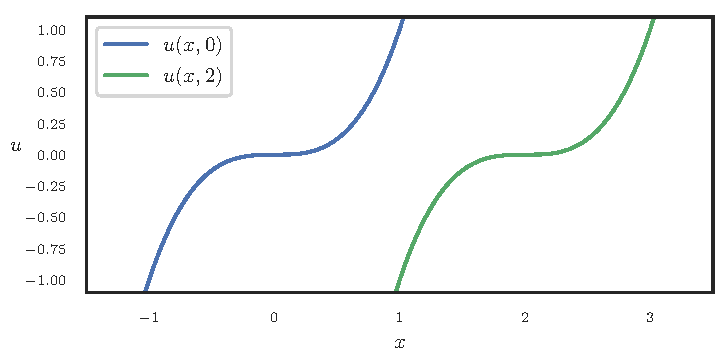
\includegraphics[width=0.95\textwidth]
                {../images/solution-transfer/simple_transport.pdf}
\end{center}
\end{frame}

\begin{frame}
\frametitle{Lagrangian Methods}
\begin{itemize}
\pause
\item Each point in physical domain is a \textbf{particle}
\pause
\item Carry value (e.g. heat, pressure, density) along characteristic curve;
  mesh travels
\pause
\item Transform PDE to family of ODEs
\end{itemize}
\end{frame}

\begin{frame}
\frametitle{Lagrangian Methods}
Add viscosity term to transport equation
\begin{equation*}
u_t + c u_x - \eps u_{xx} = 0.
\end{equation*}
\pause
Same characteristics used, \textbf{but} solution no
longer constant
\pause
\begin{equation*}
\frac{d}{dt} u(x(t), t) = \eps u_{xx}.
\end{equation*}
\end{frame}

\begin{frame}
\frametitle{Remeshing and Adaptivity}
\begin{itemize}
\item Problems caused by flow-based mesh changes
\begin{itemize}
\pause
\item Distortion
\pause
\item Tangling
\pause
\item Travel outside relevant physical domain
\end{itemize}
\pause
\item Adaptivity
\begin{itemize}
\pause
\item Dynamically focus computational effort
\pause
\item Resolve sensitive features
\end{itemize}
\end{itemize}
\end{frame}

\begin{frame}
\frametitle{Remeshing Example}
Consider
\begin{equation*}
u_t + \left[ \begin{array}{c} y^2 \\ 1 \end{array}\right] \cdot \nabla u +
  F\left(u, \nabla u\right) = 0
\end{equation*}
\pause
with cubic characteristics
\begin{equation*}
\left[ \begin{array}{c} x(t) \\ y(t) \end{array}\right] =
  \left[ \begin{array}{c} x_0 \\ y_0 \end{array}\right] +
  \frac{1}{3} \left[ \begin{array}{c} (y_0 + t)^3 - y_0^3 \\
  3t \end{array}\right].
\end{equation*}
\end{frame}

\begin{frame}
\frametitle{Remeshing Example}
\begin{center}
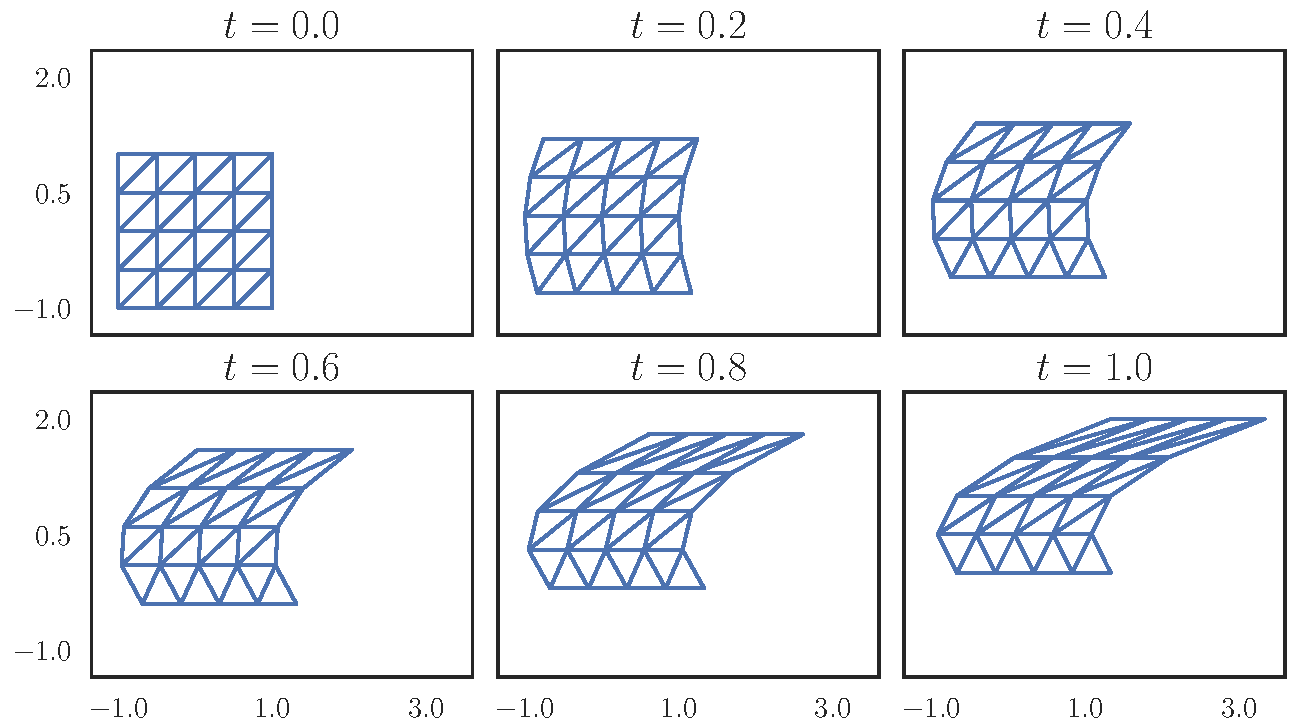
\includegraphics[width=0.95\textwidth]
                {../images/slides/mesh_distortion.pdf}
\end{center}
\end{frame}

\begin{frame}
\frametitle{Remeshing Example}
\begin{center}
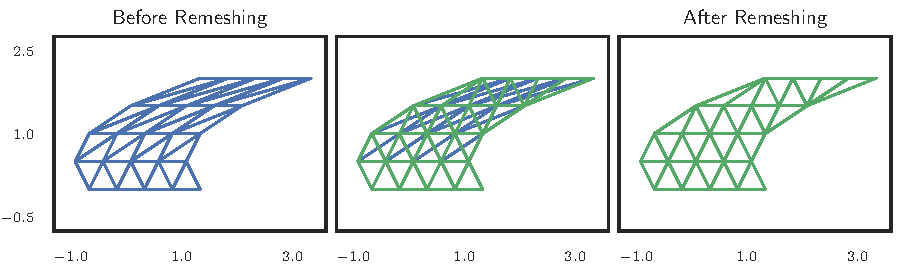
\includegraphics[width=0.95\textwidth]
                {../images/solution-transfer/distortion_remesh.pdf}
\end{center}
\end{frame}

\begin{frame}
\frametitle{Curved Meshes}
\only<1-5,7-11>{
\begin{itemize}
\item<1-5,7-11> Benefits
\begin{itemize}
\item<2-5,7-11> High-order shape functions, highly accurate solutions
\item<3-5,7-11> Low dissipation and dispersion error
\item<4-5,7-11> Greater geometric flexibility
\item<5,7-11> Fewer elements
\end{itemize}
\item<8-11> Drawbacks
\begin{itemize}
\item<9-11> Harder to implement
\item<10-11> Loss of accuracy in high degree (e.g. Runge's phenomenon)
\item<11> More challenging geometry
\end{itemize}
\end{itemize}
}
%%
\begin{center}
\includegraphics<6>[width=0.95\textwidth]
                   {../images/solution-transfer/main_figure27.pdf}
\includegraphics<12>[width=0.95\textwidth]
                    {../images/slides/not_convex.pdf}
\includegraphics<13>[width=0.95\textwidth]
                    {../images/slides/split_intersection.pdf}
\end{center}
\end{frame}

\begin{frame}
\frametitle{Curved Elements}
\begin{itemize}
\item Necessary for High-order
\pause
\item With non-linear shape functions (i.e. not straight sided), non-vertex
nodes used
\pause
\item Lagrangian method must either curve mesh or information about
flow of geometry will be lost
\end{itemize}
\end{frame}

\begin{frame}
\frametitle{Curved Elements: Necessary for High-order}
%% H/T: https://stackoverflow.com/a/4684091/1068170
\begin{center}
\includegraphics<1>[width=0.95\textwidth]
                   {../images/slides/element_distortion1.pdf}
\includegraphics<2>[width=0.95\textwidth]
                   {../images/slides/element_distortion2.pdf}
\includegraphics<3>[width=0.95\textwidth]
                   {../images/slides/element_distortion3.pdf}
\end{center}
\end{frame}

%%%%%%%%%%%%%%%%%%%%%%%
%%% CURVED ELEMENTS %%%
%%%%%%%%%%%%%%%%%%%%%%%

\begin{frame}
\centering
{\Large \bf Curved Elements}
\rule{0.82\textwidth}{1pt}
\end{frame}

\begin{frame}
\frametitle{B\'{e}zier Triangles}
\begin{itemize}
\item Image \(\mathcal{T} = b\left(\utri\right)\) of reference triangle
  under polynomial map \(b(s, t)\)
\pause
\item Barycentric
  coordinates \(\lambda_1 = 1 - s - t, \lambda_2 = s, \lambda_3 = t\)
\pause
\item Bernstein basis via trinomial expansion:
\begin{equation*}
1 = \left(\lambda_1 + \lambda_2 + \lambda_3\right)^n
\end{equation*}
\pause
\vspace*{-0.9cm}
\item Convex combination of control points
\begin{equation*}
b(s, t) = \sum_{\substack{i + j + k = n \\ i, j, k \geq 0}}
  \binom{n}{i, j, k} \lambda_1^i \lambda_2^j \lambda_3^k \;
  \bm{p}_{i, j, k}
\end{equation*}
\end{itemize}
\end{frame}

\begin{frame}
\frametitle{B\'{e}zier Triangles}
\begin{center}
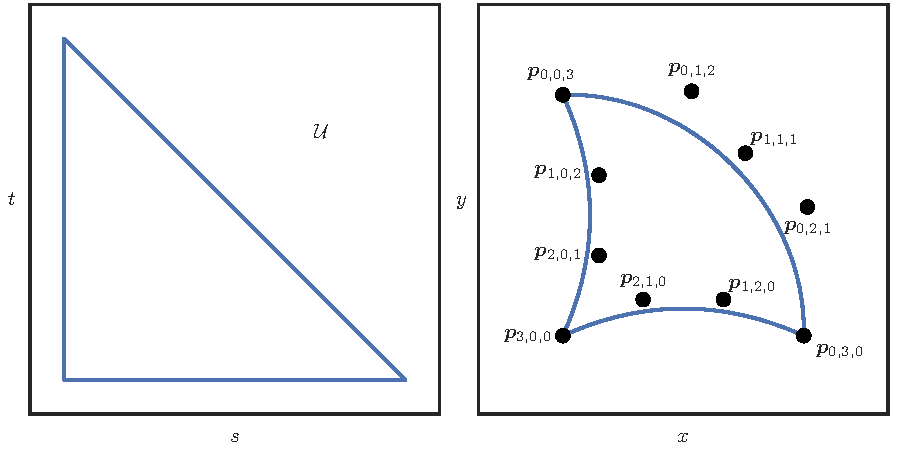
\includegraphics[width=0.95\textwidth]
                {../images/slides/main_figure31.pdf}
\end{center}
\end{frame}

\begin{frame}
\frametitle{B\'{e}zier Triangles}
\only<1-3,5-7>{
\begin{itemize}
\item<1-3,5-7> \(b(s, t)\) can be defined by data other than control net
\item<2-3,5-7> Regular grid in \(\utri\), \(\bm{u}_{i, j, k} =
  \left(\frac{j}{n}, \frac{k}{n}\right)\)
\item<3,5-7> \(b\left(\bm{u}_{i, j, k}\right) = \bm{n}_{i, j, k}\); refer to
  \(\bm{n}_{i, j, k}\) as \textbf{standard nodes}
\item<6-7> For example, taking \(\bm{n}_{i, j, k} = \delta_{(i, j, k) \;
  (i_0, j_0, k_0)}\) gives degree \(n\) shape functions on \(\utri\)
\item<7> Conversion between \(\bm{n}_{i, j, k}\) and \(\bm{p}_{i, j, k}\)
  has condition number exponential in \(n\)
\end{itemize}
}
%%
\begin{center}
\includegraphics<4>[width=0.95\textwidth]
                  {../images/preliminaries/main_figure01.pdf}
\end{center}
\end{frame}

\begin{frame}
\frametitle{Valid Element}
\begin{itemize}
\item Element \(\mathcal{T}\) is \textbf{valid} if diffeomorphic to
  \(\utri\)
\pause
\item \(b(s, t)\) bijective, i.e. Jacobian \(Db\) is everywhere invertible
\pause
\item \(\det(Db)\) positive, preserves orientation
\end{itemize}
\end{frame}

\begin{frame}
\frametitle{Inverted Element}
Consider element given by map
\begin{equation*}
b(s, t) = \lambda_1^2 \left[ \begin{array}{c} 1 \\ 0 \end{array}\right] +
\lambda_2^2 \left[ \begin{array}{c} 1 \\ 1 \end{array}\right] +
\lambda_3^2 \left[ \begin{array}{c} 0 \\ 1 \end{array}\right]
\end{equation*}
\end{frame}

\begin{frame}
\frametitle{Inverted Element}
\begin{center}
\includegraphics<1>[height=0.8\textheight]{../images/slides/boundary_leak1.pdf}
\includegraphics<2>[height=0.8\textheight]{../images/slides/boundary_leak2.pdf}
\includegraphics<3>[height=0.8\textheight]{../images/slides/boundary_leak3.pdf}
\includegraphics<4>[height=0.8\textheight]{../images/slides/boundary_leak4.pdf}
\includegraphics<5>[height=0.8\textheight]{../images/slides/boundary_leak5.pdf}
\includegraphics<6>[height=0.8\textheight]{../images/slides/boundary_leak6.pdf}
\end{center}
\end{frame}

\begin{frame}
\frametitle{Inverted Element}
\begin{center}
\includegraphics<1>[width=0.95\textwidth]
                   {../images/slides/inverted_element1.pdf}
\includegraphics<2>[width=0.95\textwidth]
                   {../images/slides/inverted_element2.pdf}
\includegraphics<3>[width=0.95\textwidth]
                   {../images/slides/inverted_element3.pdf}
\end{center}
\end{frame}

\begin{frame}
\frametitle{Shape Functions}
\only<1-2,5-8>{
\begin{itemize}
\item<1-2,5-8> Based on \(\bm{u}_{\bm{\alpha}} \in \utri\) or
  \(\bm{n}_{\bm{\alpha}} \in \mathbf{R}^2\)
  (\(\bm{\alpha}\) is a multi-index)
\item<2,5-8> \textbf{Pre-Image Basis}: \(\phi_{\bm{\alpha}}\left(
  \bm{n}_{\bm{\beta}}\right) = \widehat{\phi}_{\bm{\alpha}}\left(
  \bm{u}_{\bm{\beta}}\right) = \widehat{\phi}_{\bm{\alpha}}\left(b^{-1}\left(
  \bm{n}_{\bm{\beta}}\right)\right)\)
\item<6-8> \textbf{Global Coordinates Basis}: \(\phi_{\bm{\alpha}}\left(
  \bm{n}_{\bm{\beta}}\right) = \delta_{\bm{\alpha} \bm{\beta}}\)
\item<7-8> Element is \textbf{isoparametric} when numerical solution
  expressed in span of shape functions
\item<8> \(\operatorname{supp}(\phi) = \mathcal{T}\)
\end{itemize}
}
%%
\begin{center}
\includegraphics<3>{tikz_shape_fns1.pdf}
\includegraphics<4>{tikz_shape_fns2.pdf}
\end{center}
\end{frame}

%%%%%%%%%%%%%%%%%%%%%%%%%
%%% SOLUTION TRANSFER %%%
%%%%%%%%%%%%%%%%%%%%%%%%%

\begin{frame}
\centering
{\Large \bf Solution Transfer}
\rule{0.82\textwidth}{1pt}
\end{frame}

\begin{frame}
\frametitle{Galerkin Projection}
\begin{itemize}
\item \textbf{Given}:
\begin{itemize}
\pause
\item Donor mesh \(\mathcal{M}_D\) and target mesh \(\mathcal{M}_T\)
\pause
\item Shape function bases \(\phi_D^{(j)}\) and \(\phi_T^{(j)}\)
\pause
\item Known discrete field \(\bm{q}_D = \sum_j d_j \phi_D^{(j)}\)
\end{itemize}
\pause
\item \textbf{Want}: \(L_2\)-optimal interpolant
\(\bm{q}_T = \sum_j t_j \phi_T^{(j)}\):
\begin{equation*}
\left \lVert \bm{q}_T - \bm{q}_D \right \rVert_2 =
\min_{\bm{q} \in \mathcal{V}_T}
\left \lVert \bm{q} - \bm{q}_D \right \rVert_2
\end{equation*}
\end{itemize}
\end{frame}

\begin{frame}
\frametitle{Galerkin Projection}
\begin{center}
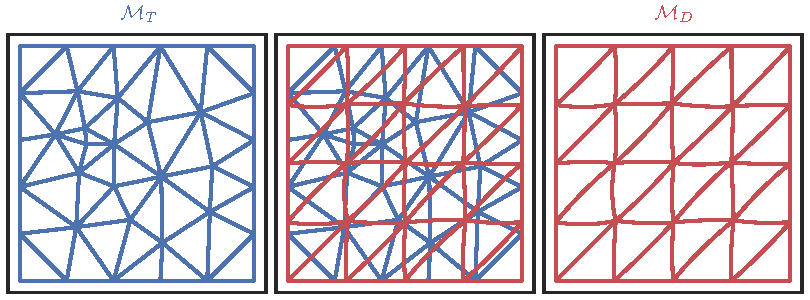
\includegraphics[width=0.95\textwidth]
                {../images/solution-transfer/main_figure00.pdf}
\end{center}
\end{frame}

\begin{frame}
\frametitle{Galerkin Projection}
Differentiating w.r.t. each \(t_j\) in
\(\bm{q}_T = \sum_j t_j \phi_T^{(j)}\) gives \textbf{weak form}
\begin{equation*}
\int_{\Omega} \bm{q}_D \phi_T^{(j)} \, dV =
  \int_{\Omega} \bm{q}_T \phi_T^{(j)} \, dV, \qquad \text{for all } j.
\end{equation*}
\pause
If \(\left(\bm{x} \mapsto 1\right) \in \mathcal{V}_T\), then \(\bm{q}_T\)
is globally \textbf{conservative}
\begin{equation*}
\int_{\Omega} \bm{q}_D \, dV =
  \int_{\Omega} \bm{q}_T \, dV.
\end{equation*}
\end{frame}

\begin{frame}
\frametitle{Linear System}
Weak form gives rise to a linear system in coefficients
\(\bm{d}\) and \(\bm{t}\):
\pause
\begin{equation*}
M_T \bm{t} = M_{TD} \bm{d}.
\end{equation*}
\end{frame}

\begin{frame}
\frametitle{Linear System}
\(M_T\) is (symmetric) mass matrix for target mesh
\begin{equation*}
\left(M_T\right)_{ij} = \int_{\Omega} \phi_T^{(i)} \phi_T^{(j)} \, dV.
\end{equation*}
\pause
Since \(\operatorname{supp}(\phi) = \mathcal{T}\),
\(M_T\) is block diagonal in DG, sparse but globally coupled in CG. \\
\pause
Integrate via substitution for \(F = \phi_T^{(i)} \phi_T^{(j)}\)
\begin{equation*}
\int_{b\left(\utri\right)} F(x, y) \, dx \, dy =
  \int_{\utri} \det(Db) F\left(x(s, t), y(s, t)\right) \, ds \, dt
\end{equation*}
and then use quadrature rule on \(\utri\).
\end{frame}

\begin{frame}
\frametitle{Linear System}
Mixed mass matrix \(M_{TD}\)
\begin{equation*}
\left(M_{TD}\right)_{ij} = \int_{\Omega} \phi_T^{(i)} \phi_D^{(j)} \, dV.
\end{equation*}
\pause
Not symmetric, nor even square; rows correspond to shape functions on target
mesh and columns to donor mesh. \\
\pause
Instead, compute entire RHS
\begin{equation*}
\left(M_{TD} \bm{d}\right)_j = \int_{\Omega} \phi_T^{(j)} \bm{q}_D \, dV.
\end{equation*}
\end{frame}

\begin{frame}
\frametitle{Common Refinement}
Given \(\phi\) supported on \(\mathcal{T}\)
\begin{equation*}
\int_{\Omega} \phi \, \bm{q}_D \, dV
  \onslide<2->{= \int_{\mathcal{T}} \phi \, \bm{q}_D \, dV}
  \onslide<3->{= \sum_{\mathcal{T}' \in \mathcal{M}_D}
    \int_{\mathcal{T} \cap \mathcal{T}'} \phi
    \left.\bm{q}_D\right|_{\mathcal{T}'} \, dV}
\end{equation*}
\onslide<4->{\noindent
In CG, \(\bm{q}_D\) need not be differentiable across elements and in
DG \(\bm{q}_D\) need not even be continuous
}
\end{frame}

\begin{frame}
\frametitle{Common Refinement}
\begin{center}
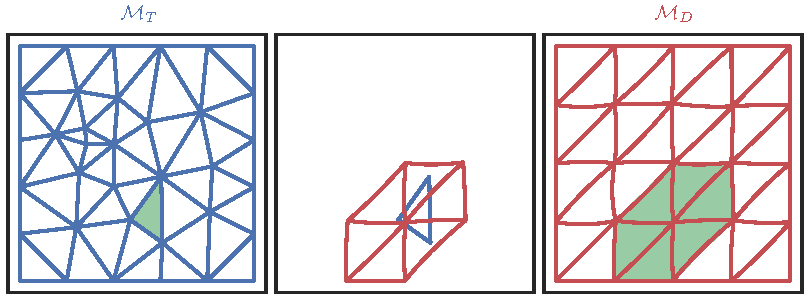
\includegraphics[width=0.95\textwidth]
                {../images/solution-transfer/main_figure02.pdf}
\end{center}
\end{frame}

\begin{frame}
\frametitle{Common Refinement}
\begin{itemize}
\item Three subproblems:
\begin{itemize}
\pause
\item Intersecting Curved Elements: \(\mathcal{T} \cap \mathcal{T}'\)
\pause
\item Advancing Front: \(\left(\mathcal{T}, \mathcal{T}'\right) \in
  \mathcal{M}_T \times \mathcal{M}_D\)
\pause
\item Integration over Curved Polygons:
  \(\displaystyle \int_{\mathcal{T} \cap \mathcal{T}'} F \, dV\)
\end{itemize}
\end{itemize}
\end{frame}

\begin{frame}
\frametitle{Intersecting Curved Elements}
\begin{itemize}
\pause
\item Find all points where edges intersect
\pause
\item \(\textcolor{seaborn-blue}{\mathcal{T}_0} =
  \textcolor{seaborn-blue}{b_0}\left(\utri\right)\),
  \(\partial \textcolor{seaborn-blue}{\mathcal{T}_0} =
  \textcolor{seaborn-blue}{E_0} \cup \textcolor{seaborn-blue}{E_1} \cup
  \textcolor{seaborn-blue}{E_2}\)
\item \(\textcolor{seaborn-green}{\mathcal{T}_1} =
  \textcolor{seaborn-green}{b_1}\left(\utri\right)\),
  \(\partial \textcolor{seaborn-green}{\mathcal{T}_1} =
  \textcolor{seaborn-green}{E_3} \cup \textcolor{seaborn-green}{E_4} \cup
  \textcolor{seaborn-green}{E_5}\)
\pause
\item Determine which curve is interior at each intersection
\pause
\item Track parameter values at each intersection and combine
  into boundary of \textbf{curved polygon}
\pause
\item \(\mathcal{P} = \textcolor{seaborn-blue}{\mathcal{T}_0} \cap
  \textcolor{seaborn-green}{\mathcal{T}_1}\), \(\partial \mathcal{P}\)
  defined by segments of edges from \(\textcolor{seaborn-blue}{\mathcal{T}_0}\)
  and \(\textcolor{seaborn-green}{\mathcal{T}_1}\)
\end{itemize}
\end{frame}

\begin{frame}
\frametitle{Intersecting Curved Elements}
\begin{center}
\includegraphics<1>[width=0.95\textwidth]{../images/slides/main_figure32.pdf}
\includegraphics<2>[width=0.95\textwidth]{../images/slides/main_figure33.pdf}
\includegraphics<3>[width=0.95\textwidth]{../images/slides/main_figure34.pdf}
\includegraphics<4>[width=0.95\textwidth]{../images/slides/main_figure35.pdf}
\includegraphics<5>[width=0.95\textwidth]{../images/slides/main_figure36.pdf}
\includegraphics<6>[width=0.95\textwidth]{../images/slides/main_figure37.pdf}
\end{center}
\end{frame}

\begin{frame}
\frametitle{Intersecting Curved Elements}
\begin{itemize}
\item \(\mathcal{P} = \textcolor{seaborn-blue}{\mathcal{T}_0} \cap
  \textcolor{seaborn-green}{\mathcal{T}_1}\)
\item \(\partial \mathcal{P} = \textcolor{seaborn-green}{E_3\left(\left[
  \frac{1}{6}, \frac{3}{4}\right]\right)} \cup
  \textcolor{seaborn-blue}{E_1\left(\left[\frac{1}{8}, 1\right]\right)} \cup
  \textcolor{seaborn-blue}{E_2\left(\left[0, \frac{7}{9}\right]\right)}\)
\end{itemize}
\end{frame}

\begin{frame}
\frametitle{Advancing Front}
\only<1-2,4-7,9-10,12->{
\begin{itemize}
\item<1-2,4-7,9-10,12-> Find all pairs \(\mathcal{T}\), \(\mathcal{T}'\) of
  intersecting target and donor elements
\item<2,4-7,9-10,12-> Fix target element \(\mathcal{T}\), perform brute-force search
\begin{itemize}
\item<5-7,9-10,12-> \(\bigO{\left|\mathcal{M}_D\right|}\)
\item<6-7,9-10,12-> \(\bigO{1}\) in typical ALE, though acts as CFL
\end{itemize}
\item<7,9-10,12-> Use donor mesh connectivity to perform breadth first search
  for neighbors \(\mathcal{N}_{\mathcal{T}}\) that intersect
  \(\mathcal{T}\) (as well as a one element buffer)
\item<10,12-> Neighbors of \(\mathcal{T}\) can find one matching donor element
  among \(\mathcal{N}_{\mathcal{T}}\) in
  \(\bigO{\left|\mathcal{N}_{\mathcal{T}}\right|} = \bigO{1}\)
\item<13-> Total \(\bigO{\left|\mathcal{M}_D\right| +
  \left|\mathcal{M}_T\right|}\)
\end{itemize}
}
%%
\begin{center}
\includegraphics<3>[width=0.95\textwidth]
                   {../images/solution-transfer/main_figure13.pdf}
\includegraphics<8>[width=0.95\textwidth]
                   {../images/solution-transfer/main_figure14.pdf}
\includegraphics<11>[width=0.95\textwidth]
                    {../images/solution-transfer/main_figure15.pdf}
\end{center}
\end{frame}

\begin{frame}
\frametitle{Integration over Curved Polygons}
\begin{equation*}
\int_{\mathcal{P}} F(x, y) \, dV, \qquad \mathcal{P} = \mathcal{T}_0 \cap
  \mathcal{T}_1, \qquad F = \phi_0 \, \phi_1
\end{equation*}
\end{frame}

\begin{frame}
\frametitle{Integrate via Polygonal Approximation}
\begin{center}
\includegraphics<1>[width=0.95\textwidth]
                   {../images/slides/polygon_vs_curved1.pdf}
\includegraphics<2>[width=0.95\textwidth]
                   {../images/slides/polygon_vs_curved2.pdf}
\includegraphics<3>[width=0.95\textwidth]
                   {../images/slides/polygon_vs_curved3.pdf}
\includegraphics<4>[width=0.95\textwidth]
                   {../images/slides/polygon_vs_curved4.pdf}
\includegraphics<5>[width=0.95\textwidth]
                   {../images/slides/polygon_vs_curved5.pdf}
\includegraphics<6>[width=0.95\textwidth]
                   {../images/slides/polygon_vs_curved6.pdf}
\end{center}
\end{frame}

\begin{frame}
\frametitle{Integrate via Polygonal Quadrature}
\begin{itemize}
\item Polygonal quadrature rules not in wide use
\pause
\item \(\mathcal{P}\) has curved edges
\pause
\item Transfinite interpolation or mean value coordinates
\begin{itemize}
\pause
\item Maps from (straight sided) reference domain, but increase degree or
  are not bijective
\end{itemize}
\end{itemize}
\end{frame}

\begin{frame}
\frametitle{Integrate via Tessellation}
\begin{itemize}
\item Triangular quadrature rules simple and well established
\pause
\item Tessellate \(\mathcal{P}\) into disjoint union of B\'{e}zier triangles
\end{itemize}
\end{frame}

\begin{frame}
\frametitle{Integrate via Tessellation}
\begin{center}
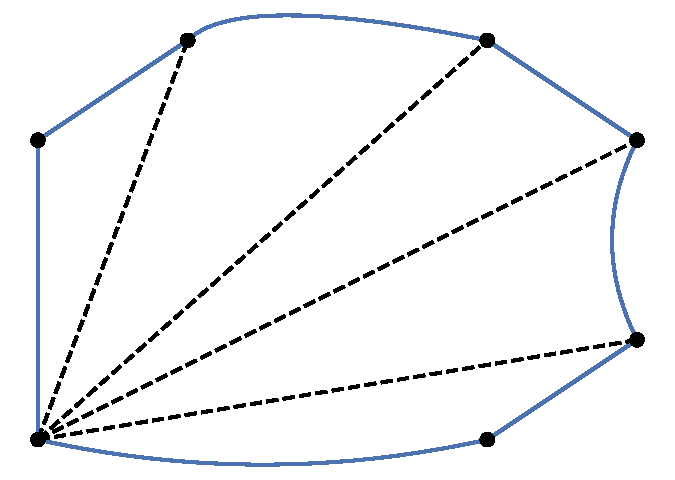
\includegraphics[width=0.95\textwidth]
                {../images/solution-transfer/main_figure11.pdf}
\end{center}
\end{frame}

\begin{frame}
\frametitle{Integrate via Tessellation}
\begin{itemize}
\item Not clear if an arbitrary curved polygon
\textbf{can} be tessellated without introducing interior nodes
\pause
\item Need to check if diagonals cross edges; even worse if diagonals are
  also curved
\pause
\item If diagonals are valid, high degree B\'{e}zier triangles
  need interior control points introduced that don't cause triangle
  to invert
\end{itemize}
\end{frame}

\begin{frame}
\frametitle{Integrate via Tessellation}
\only<1,3-7>{
\begin{itemize}
\item<1,3-7> Tessellate with inverted B\'{e}zier triangles?
\item<4-7> E.g. tessellation of \(\mathcal{P}\) contains inverted
  \(\mathcal{T}_2 = b\left(\utri\right)\), then numerically
  integrate
\begin{equation*}
\int_{\mathcal{T}_2} \phi_0 \phi_1 \, dx \, dy =
  \int_{\utri} \left|\det(Db)\right| \left(\phi_0 \circ b\right)
  \left(\phi_1 \circ b\right) \, ds \, dt
\end{equation*}
\item<5-7> \(\left|\det(Db)\right|\) non-smooth, bad for quadrature
\item<6-7> If \(\phi_0\) from pre-image basis, then \(\phi_0 \circ b =
  \widehat{\phi}_0 \circ b_0^{-1} \circ b\)
\item<7> \(\mathcal{T}_2\) inverted, \(b(s, t) \not\in \mathcal{P}\) is
  possible but \(b_0^{-1}\) need not need be defined outside of
  \(\mathcal{T}_0\)
\end{itemize}
}
%%
\begin{center}
\includegraphics<2>[height=0.8\textheight]
                   {../images/solution-transfer/main_figure16.pdf}
\end{center}
\end{frame}

\begin{frame}
\frametitle{Integrate via Green's Theorem}
\begin{itemize}
\item Horizontal antiderivative \(H\) and vertical antiderivative \(V\) s.t.
  \(H_x = V_y = F\)
\pause
\item \(H(0, y) \equiv V(x, 0) \equiv 0\) for uniqueness (needed
  to evaluate)
\pause
\item If \(\partial\mathcal{P} = C_1 \cup \cdots \cup C_n\),
  since \(2F = H_x + V_y\) Green's gives
\begin{equation*}
\int_{\mathcal{P}} 2 F \, dV =
\oint_{\partial \mathcal{P}} H \, dy - V \, dx =
\sum_j \int_{C_j} H \, dy - V \, dx
\end{equation*}
\pause
\vspace*{-0.6cm}
\item Each \(C\) given by \(x(r), y(r)\),
  1D quadrature on unit interval of
\begin{equation*}
G(r) = H(x(r), y(r)) y'(r) - V(x(r), y(r)) x'(r)
\end{equation*}
\end{itemize}
\end{frame}

\begin{frame}
\frametitle{Integrate via Green's Theorem}
\begin{itemize}
\item How to evaluate \(H(x(r), y(r))\)?
\pause
\item Fundamental theorem of calculus
\begin{equation*}
H\left(\alpha, \beta\right) =
  H\left(\alpha, \beta\right) - H\left(0, \beta\right) =
  \int_0^{\alpha} F\left(x, \beta\right) \, dx
\end{equation*}
\pause
\vspace*{-0.6cm}
\item Quadrature points \(F\left(x_j, \beta\right)\) may fall outside
  \(\mathcal{P}\), so pre-image basis cannot be used
\pause
\item Global coordinates basis means \(F\) is a polynomial on
  \(\mathbf{R}^2\), so quadrature is exact
\end{itemize}
\end{frame}

\begin{frame}
\frametitle{Numerical Experiments}
\only<1,3-9>{
\begin{itemize}
\item<1,3-9> Three meshes (\(p = 1, 2, 3\))
\item<4-9> Three functions
\begin{itemize}
\item<5-9> \(\zeta_1(x, y) = 5 y^3 + x^2 + 2y + 3\)
\item<6-9> \(\zeta_2(x, y) = \exp\left(x^2\right) + 2y\)
\item<7-9> \(\zeta_3(x, y) = \sin(x) + \cos(y)\)
\end{itemize}
\item<8-9> Nodal interpolant
\(\displaystyle \bm{q}_D = \sum_j \zeta\left(\bm{n}_j\right) \phi_D^{(j)}\)
\item<9> Expect \(\bigO{h^{p + 1}}\) errors
\end{itemize}
}
%%
\begin{center}
\includegraphics<2>{../images/solution-transfer/main_figure30.pdf}
\end{center}
\end{frame}

\begin{frame}
\frametitle{Numerical Experiments}
\begin{center}
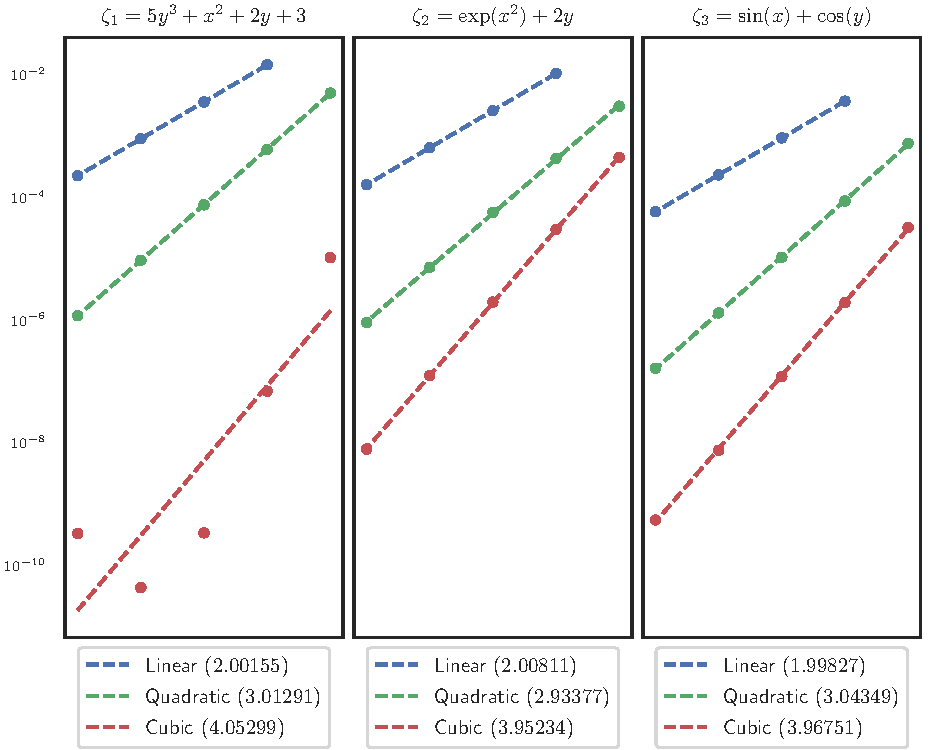
\includegraphics[height=0.8\textheight]
                {../images/solution-transfer/main_figure25.pdf}
\end{center}
\end{frame}

%%%%%%%%%%%%%%%%%%%%%%%%%%%%%%%%%%%%%%%%%%%%%%%%%%%%%
%%% ILL-CONDITIONED B\'{E}ZIER CURVE INTERSECTION %%%
%%%%%%%%%%%%%%%%%%%%%%%%%%%%%%%%%%%%%%%%%%%%%%%%%%%%%

\begin{frame}
\centering
{\Large \bf Ill-conditioned B\'{e}zier Curve Intersection}
\rule{0.82\textwidth}{1pt}
\end{frame}

\begin{frame}
\frametitle{Ill-Conditioned Intersections}
\includegraphics<1>[width=0.95\textwidth]
                   {../images/bezier-intersection/main_figure22.pdf}
\includegraphics<2>[width=0.95\textwidth]
                   {../images/bezier-intersection/main_figure23.pdf}
\end{frame}

\begin{frame}
\frametitle{Ill-Conditioned Intersections}
\begin{itemize}
\item Edges are B\'{e}zier curves, e.g. \(b(r, 0) = \sum_{j = 0}^n
  \binom{n}{j} (1 - r)^{n - j} r^j \; \bm{p}_{n - j, j, 0}\)
\pause
\item Tangent intersection equivalent to double root of polynomial,
  i.e. condition number is infinite
\pause
\item Random pair of meshes, ``almost tangent'' intersections increasingly
  frequent as \(h \longrightarrow 0^+\)
\end{itemize}
\end{frame}

%% H/T: https://stackoverflow.com/a/3594456
\begin{frame}
\frametitle{Intersection Algorithm}
\only<1,3-4,6-7,9-10,12-13>{
\begin{itemize}
\item<1,3-4,6-7,9-10,12-13> {\color<13>{fg!20} Bounding box check}
\item<4,6-7,9-10,12-13> {\color<13>{fg!20} Curve subdivision}
\item<7,9-10,12-13> {\color<13>{fg!20} Check subdivided pairs}
\item<10,12-13> {\color<13>{fg!20} Subdivide until ``almost'' linear}
\item<13> Use intersection of lines as seed for Newton's method
\end{itemize}
}
%%
\begin{center}
\includegraphics<2>[width=0.95\textwidth]
                   {../images/bezier-intersection/bbox_check.pdf}
\includegraphics<5>[width=0.95\textwidth]
                   {../images/bezier-intersection/subdivide_curve.pdf}
\includegraphics<8>[width=0.95\textwidth]
                   {../images/bezier-intersection/subdivision_process.pdf}
\includegraphics<11>[width=0.95\textwidth]
                    {../images/bezier-intersection/subdivision_linearized.pdf}
\end{center}
\end{frame}

\begin{frame}
\frametitle{Newton's Method}
\begin{itemize}
\item B\'{e}zier curves \(b_0(s), b_1(t)\) map into \(\mathbf{R}^2\)
\pause
\item Residual \(F(s, t) = b_0(s) - b_1(t)\), Jacobian \(J =
\left[ \begin{array}{c c} b_0'(s) & -b_1'(t) \end{array}\right]\)
\pause
\item Newton's:
\begin{equation*}
\left[ \begin{array}{c} s_{n + 1} \\ t_{n + 1} \end{array}\right] =
\left[ \begin{array}{c} s_n \\ t_n \end{array}\right] -
J_n^{-1} F_n
\end{equation*}
\pause
\item At tangent intersections, \(J\) is exactly singular
\pause
\item At ill-conditioned intersections, \(J\) is almost singular and
  evaluation of \(F\) is typically ill-conditioned as well
\end{itemize}
\end{frame}

\begin{frame}
\frametitle{Modified Newton's Method}
\begin{itemize}
\item Sources of error:
\begin{itemize}
\pause
\item Evaluation of \(F\)
\pause
\item Evaluation of \(J\)
\pause
\item Solution of \(J \bm{y} = F\)
\end{itemize}
\pause
\item Can improve accuracy of Newton's method by using extended
  precision for evaluation of \(F\), even in presence of
  inaccurate \(J\) and unstable solve
\begin{itemize}
\pause
\item Tisseur (2001) showed this generically and applied to iterative
  refinement for generalized eigenvalue problem
\end{itemize}
\end{itemize}
\end{frame}

%%%%%%%%%%%%%%%%%%%%%%%%%%%%%%
%%% COMPENSATED EVALUATION %%%
%%%%%%%%%%%%%%%%%%%%%%%%%%%%%%

\begin{frame}
\centering
{\Large \bf Compensated Evaluation}
\rule{0.82\textwidth}{1pt}
\end{frame}

\begin{frame}
\frametitle{Compensated Algorithms}
\begin{itemize}
\item Error-free transform (EFT):
\begin{itemize}
\pause
\item Problem \(f(x)\), algorithm computes \(\widehat{f}\)
\pause
\item EFT modifies algorithm to also produce error \(\widehat{e}\)
  so that \\ \(f(x) = \widehat{f} + \widehat{e}\)
\pause
\item Error is \textbf{exact}, hence ``error-free''
\end{itemize}
\pause
\item \textbf{Compensated} algorithm uses \(\widehat{f} \oplus \widehat{e}\);
  better approximation of \(f(x)\) than \(\widehat{f}\) (usually)
\end{itemize}
\end{frame}

\begin{frame}
\frametitle{EFT for Addition}
\begin{itemize}
\item \(\mathtt{TwoSum}(a, b) = \left[S, \sigma\right]\)
\pause
\item \(a + b = S + \sigma\)
\pause
\item Algorithm:
\begin{itemize}
\pause
\item \(S = a \oplus b\)
\pause
\item \(\mathtt{almost\_b} = S \ominus a\)
\pause
\item \(\sigma = (a \ominus (S \ominus \mathtt{almost\_b}))
  \oplus (b \ominus \mathtt{almost\_b})\)
\end{itemize}
\end{itemize}
\end{frame}

\begin{frame}
\frametitle{EFT for Multiplication}
\begin{itemize}
\item \(\mathtt{TwoProd}(a, b) = \left[P, \pi\right]\)
\pause
\item \(a \times b = P + \pi\)
\pause
\item Algorithm:
\begin{itemize}
\pause
\item \(P = a \otimes b\)
\pause
\item \(\pi = \mathtt{FusedMultiplyAdd}(a, b, -P)\)
\end{itemize}
\pause
\item \textbf{Not possible} to apply this to \(\oslash\)
\end{itemize}
\end{frame}

\begin{frame}
\frametitle{B\'{e}zier Curve Evaluation}
\begin{itemize}
\item \(p(s) = \binom{n}{0} (1 - s)^n \cdot b_0 +
  \binom{n}{1} (1 - s)^{n - 1} s \cdot b_1 + \cdots\)
\pause
\item de Casteljau Algorithm:
\begin{itemize}
\pause
\item \(\widehat{\bm{b}}^{(n)} = \bm{b}\), \(\widehat{r} = 1 \ominus s\)
\pause
\item \(\widehat{\bm{b}}^{(k)} = \left(\widehat{r} \otimes
  \widehat{\bm{b}}_{0:k}^{(k + 1)}\right) \oplus \left(s \otimes
  \widehat{\bm{b}}_{1:k + 1}^{(k + 1)}\right)\)
\pause
\item \(\widehat{p} = \widehat{\bm{b}}_0^{(0)}\)
\end{itemize}
\pause
\item Only uses \(\oplus\), \(\ominus\) and \(\otimes\)
\end{itemize}
\end{frame}

\begin{frame}
\frametitle{Compensated de Castlejau}
\begin{itemize}
\item Use EFT for \(\oplus\), \(\ominus\) and \(\otimes\)
\pause
\item Track errors and combine them progressively
\pause
\item Test polynomial \(p(s) = (s - 1)\left(s - \frac{3}{4}\right)^7\);
  evaluation at \(s = \frac{3}{4}\) has infinite condition, very
  ill-conditioned nearby
\end{itemize}
\end{frame}

\begin{frame}
\frametitle{Compensated de Castlejau}
\only<1>{
\begin{equation*}
\frac{\left|p(s) - \mathtt{DeCasteljau}\left(p, s\right)\right|}{
  \left|p(s)\right|} \leq \cond{p, s} \cdot \bigO{\mach}
\end{equation*}
}
%%
\only<3>{
\begin{equation*}
\frac{\left|p(s) - \mathtt{CompDeCasteljau}\left(p, s\right)\right|}{
  \left|p(s)\right|} \leq \bigO{\mach} + \cond{p, s} \cdot \bigO{\mach^2}
\end{equation*}
}
%%
\only<5>{
\begin{equation*}
\frac{\left|p(s) - \mathtt{CompDeCasteljauK}\left(p, s\right)\right|}{
  \left|p(s)\right|} \leq \bigO{\mach} + \cond{p, s} \cdot \bigO{\mach^K}
\end{equation*}
}
%%
\begin{center}
\includegraphics<2>[height=0.8\textheight]
                   {../images/slides/de_casteljau_rel_error1.pdf}
\includegraphics<4>[height=0.8\textheight]
                   {../images/slides/de_casteljau_rel_error2.pdf}
\includegraphics<6>[height=0.8\textheight]
                   {../images/slides/de_casteljau_rel_error3.pdf}
\includegraphics<7>[height=0.8\textheight]
                   {../images/slides/de_casteljau_rel_error4.pdf}
\end{center}
\end{frame}

%%%%%%%%%%%%%%%%%%%%%%%%%%%%%%%%%%%%%%%%%%
%%% MODIFIED NEWTON'S FOR INTERSECTION %%%
%%%%%%%%%%%%%%%%%%%%%%%%%%%%%%%%%%%%%%%%%%

\begin{frame}
\centering
{\Large \bf Modified Newton's for Intersection}
\rule{0.82\textwidth}{1pt}
\end{frame}

\begin{frame}
\frametitle{Polynomial Roots}
\begin{itemize}
\item \(p(s)\) written in Bernstein-B\'{e}zier form
\pause
\item Newton: \(s_{n + 1} = s_n - \frac{p(s_n)}{p'(s_n)}\)
\pause
\item Three algorithms
\begin{itemize}
\pause
\item \texttt{DNewtonBasic}: \texttt{DeCasteljau} for residual \(p(s)\)
  and Jacobian \(p'(s)\)
\pause
\item \texttt{DNewtonAccurate}: \texttt{CompDeCasteljau} for residual,
  \texttt{DeCasteljau} for Jacobian
\pause
\item \texttt{DNewtonFull}: \texttt{CompDeCasteljau} for residual and Jacobian
\end{itemize}
\end{itemize}
\end{frame}

\begin{frame}
\frametitle{Polynomial Roots}
\begin{itemize}
\item Test problem; need coefficients that can be exactly represented
\pause
\item \(p(s) = (1 - 5s)^n + 2^{30} (1 - 3s)^n\), \(n\) odd
\pause
\item Root \(\displaystyle \alpha = \frac{1 + 2^{30/n}}{5 + 3 \cdot 2^{30/n}}
  \in \left[\frac{1}{4}, \frac{1}{3}\right]\)
\end{itemize}
\end{frame}

\begin{frame}
\frametitle{Polynomial Roots}
\begin{center}
\includegraphics<1>[height=0.8\textheight]
                   {../images/slides/newton_de_casteljau1.pdf}
\includegraphics<2>[height=0.8\textheight]
                   {../images/slides/newton_de_casteljau2.pdf}
\includegraphics<3>[height=0.8\textheight]
                   {../images/slides/newton_de_casteljau3.pdf}
\end{center}
\end{frame}

\begin{frame}
\frametitle{B\'{e}zier Curve Intersection}
\begin{itemize}
\item \(F(s, t) = b_0(s) - b_1(t)\)
\pause
\item Evaluate \(x_0(s), y_0(s), x_1(t), y_1(t)\) via de Casteljau
\pause
\item Modify Newton's method by using ``extended precision'' (i.e.
  compensated method) for \(\widehat{F}\)
\end{itemize}
\end{frame}

\begin{frame}
\frametitle{Compensated Residual}
\begin{itemize}
\item \(\widehat{F} = \left[ \begin{array}{c} \widehat{x} \\
    \widehat{y} \end{array}\right]\)
\pause
\item \(\widehat{x} = \mathtt{CompDeCasteljau}\left(x_0, s\right) \ominus
  \mathtt{CompDeCasteljau}\left(x_1, t\right)\)
\pause
\item Fails; \(x_0(s), x_1(t)\) may not be near zero, e.g.
  \(\widehat{x}_0 \oplus \widehat{e}_0 = \widehat{x}_0\)
\pause
\item Instead use EFT \(x_j = \widehat{x}_j + \widehat{e}_j\), then
  combine big with big and small with small
\pause
\item Compensated addition (via \texttt{TwoSum})
  \(\widehat{x}_0 - \widehat{x}_1 = D + \widehat{e}_2\)
\pause
\item Compensation term \(\tau = \left(\widehat{e}_0 \ominus
  \widehat{e}_1\right) \oplus \widehat{e}_2\)
\pause
\item Computed residual \(D \oplus \tau\)
\end{itemize}
\end{frame}

\begin{frame}
\frametitle{Modified Newton's in Practice}
\begin{equation*}
F(s, t) = \left[ \begin{array}{c} 2(4s^2 - 1) \\ (2s - 1)^2 + 1
\end{array}\right] - \left[ \begin{array}{c} 4(4t^2 - 1) \\ 4(2t - 1)^2 + 1
\end{array}\right]
\end{equation*}
\pause
\begin{center}
Triple root at \(F\left(\frac{1}{2}, \frac{1}{2}\right)\)
\end{center}
\pause
\begin{center}
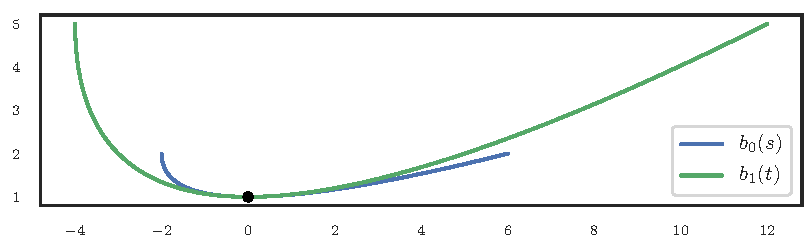
\includegraphics[width=0.95\textwidth]
                {../images/slides/tangent_intersection.pdf}
\end{center}
\end{frame}

\begin{frame}
\frametitle{Modified Newton's in Practice}
\begin{center}
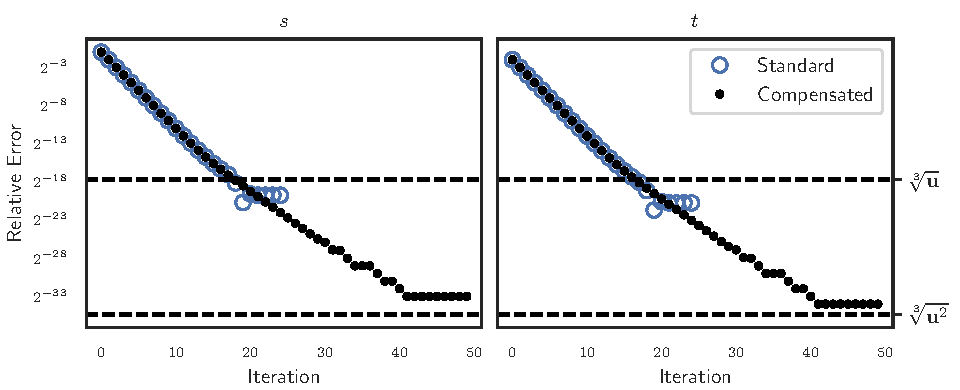
\includegraphics[width=0.95\textwidth]
                {../images/compensated-newton/newton_linear_converge.pdf}
\end{center}
\end{frame}

\begin{frame}
\frametitle{Modified Newton's in Practice}
\begin{equation*}
G(s, t) = \left[ \begin{array}{c} x_0(s) - r \\ y_0(s) + \frac{1}{r}
\end{array}\right] - \left[ \begin{array}{c} x_1(t) \\ y_1(t) + \frac{1}{r}
\end{array}\right]
\end{equation*}
\pause
\begin{center}
Approaches triple root as \(r \longrightarrow 0^+\),
  \(F\left(\frac{1 + \sqrt{r}}{2}, \frac{2 + \sqrt{r}}{4}\right)\)
\end{center}
\end{frame}

\begin{frame}
\frametitle{Modified Newton's in Practice}
\begin{center}
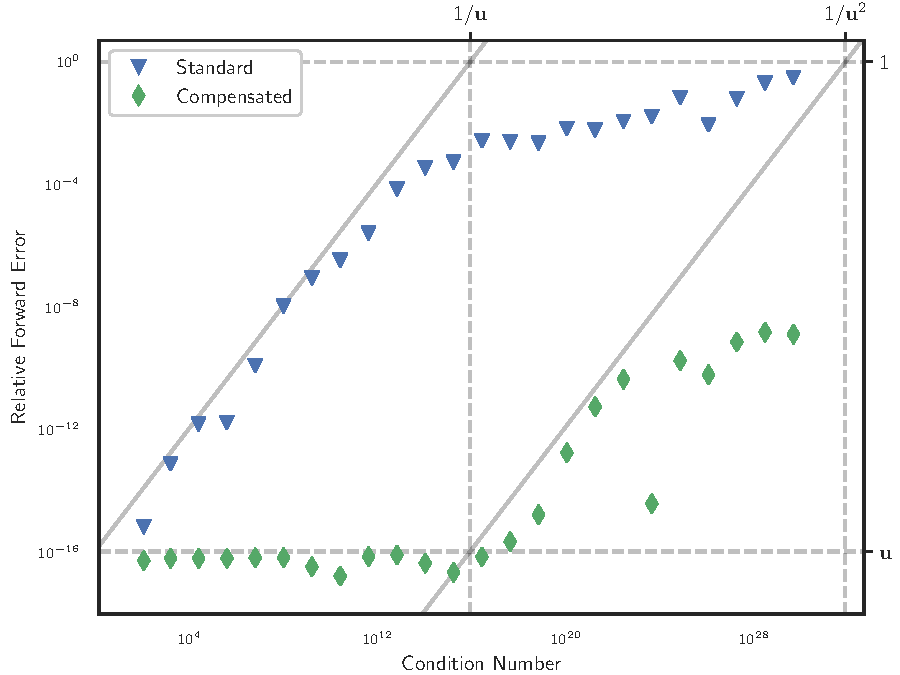
\includegraphics[height=0.8\textheight]
                {../images/compensated-newton/almost_tangent.pdf}
\end{center}
\end{frame}

%%%%%%%%%%%%%%%%%%
%%% Conclusion %%%
%%%%%%%%%%%%%%%%%%

\begin{frame}
\centering
{\Large \bf Conclusion}
\rule{0.82\textwidth}{1pt}
\end{frame}

\begin{frame}
\frametitle{Conclusion}
\begin{itemize}
\pause
\item \textbf{Solution Transfer on Curved Meshes}
\begin{itemize}
\pause
\item Conservative \(L_2\)-optimal interpolation; split
  \(\displaystyle \int_{\Omega}\) into \(\displaystyle \sum \int_{\mathcal{T}
  \cap \mathcal{T}'}\) where integrand is smooth
\pause
\item Intersecting Curved Elements: \(\mathcal{T} \cap \mathcal{T}'\)
\pause
\item Advancing Front: \(\left(\mathcal{T}, \mathcal{T}'\right) \in
  \mathcal{M}_T \times \mathcal{M}_D\)
\pause
\item Integration over Curved Polygons:
  \(\displaystyle \int_{\mathcal{T} \cap \mathcal{T}'} F \, dV\)
\end{itemize}
\pause
\item \textbf{Ill-conditioned B\'{e}zier Curve Intersection}
\begin{itemize}
\pause
\item Compensated de Castaljau for evaluation of B\'{e}zier curves
\pause
\item Modified Newton's method; computes residual \(F(s, t)\) as
  if in extended precision
\end{itemize}
\end{itemize}
\end{frame}

\begin{frame}
\frametitle{Future Work}
\begin{itemize}
\pause
\item Valid tessellation of curved polygons
\pause
\item Integrand \(F = \phi_0 \phi_1\) is polynomial in \(x, y\), could
  compute coefficients and use them to compute \(H, V\) without
  FTC, without points outside \(\mathcal{P}\)
\pause
\item Solution transfer in \(\mathbf{R}^3\); integrate via Stoke's theorem,
  geometry is greatest challenge
\pause
\item Parallelize via domain decomposition (inherently local)
\end{itemize}
\end{frame}

\end{document}
